\chapter{Caracterización Morfológica y Composicional}
\label{MEB}
Se eligieron las muestras con x=0.0, 0.5, 2.5 y 4.5 para realizar la
caracterización morfológica y composicional con aumento desde los 2k a los 90k,
con el fin de ver la variación en la microestructura a medida que se aumentaba
la inclusión de \ce{Fe^{3+}}, además se obtuvieron micrografías con EDX para
determinar las características superficiales de los materiales.\\

\begin{figure}[h]
    \centering%

    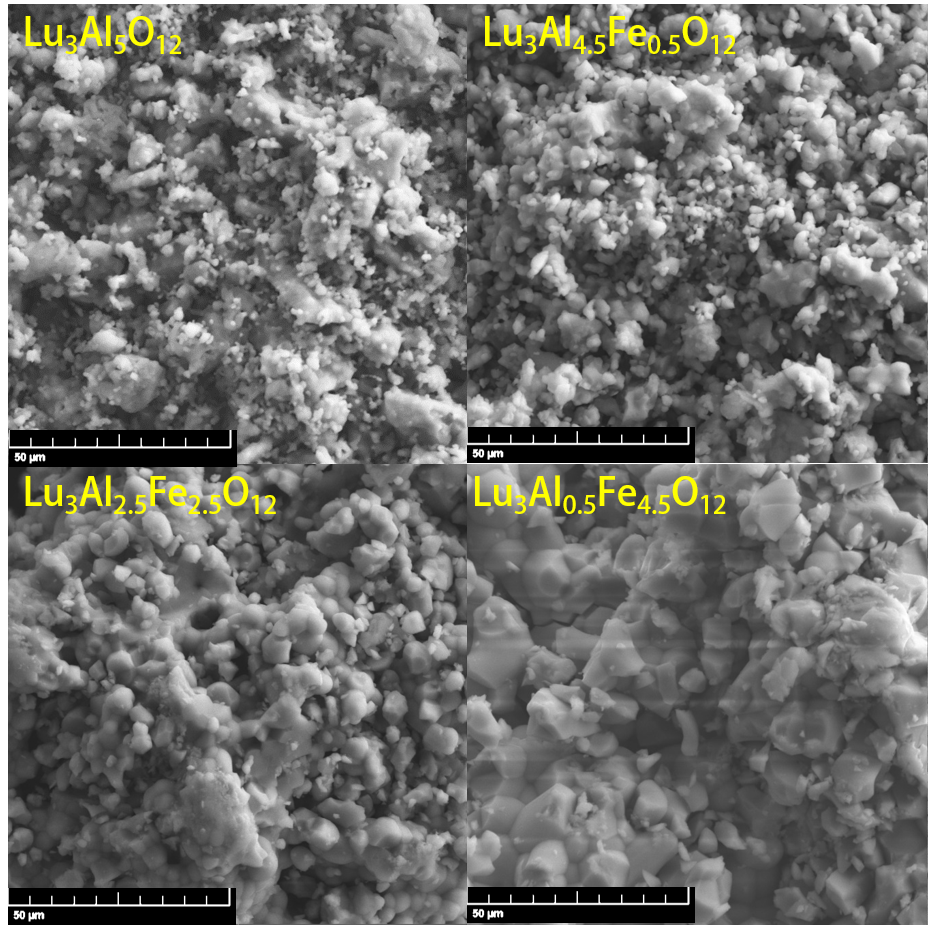
\includegraphics[width=12cm]{Kap5/sec20k.png}%
    \caption{Micrografías con electrones secundarios a 20.000 aumentos para los
    materiales \ce{Lu3Al_{5-X}Fe_{x}O12}:\ce{Ce^{3+}} con x=0.0, 0.5, 2.5
    }\label{fig:sec20}
\end{figure}

En la Figura \ref{fig:sec20} se presentan las micrografías obtenidas con
electrones
secundarios que proporcionan información topográfica de cada
muestra, en donde, se observó la formación de agregados con formas irregulares
y bordes bien definidos.\\

\begin{figure}[h]
    \centering%

    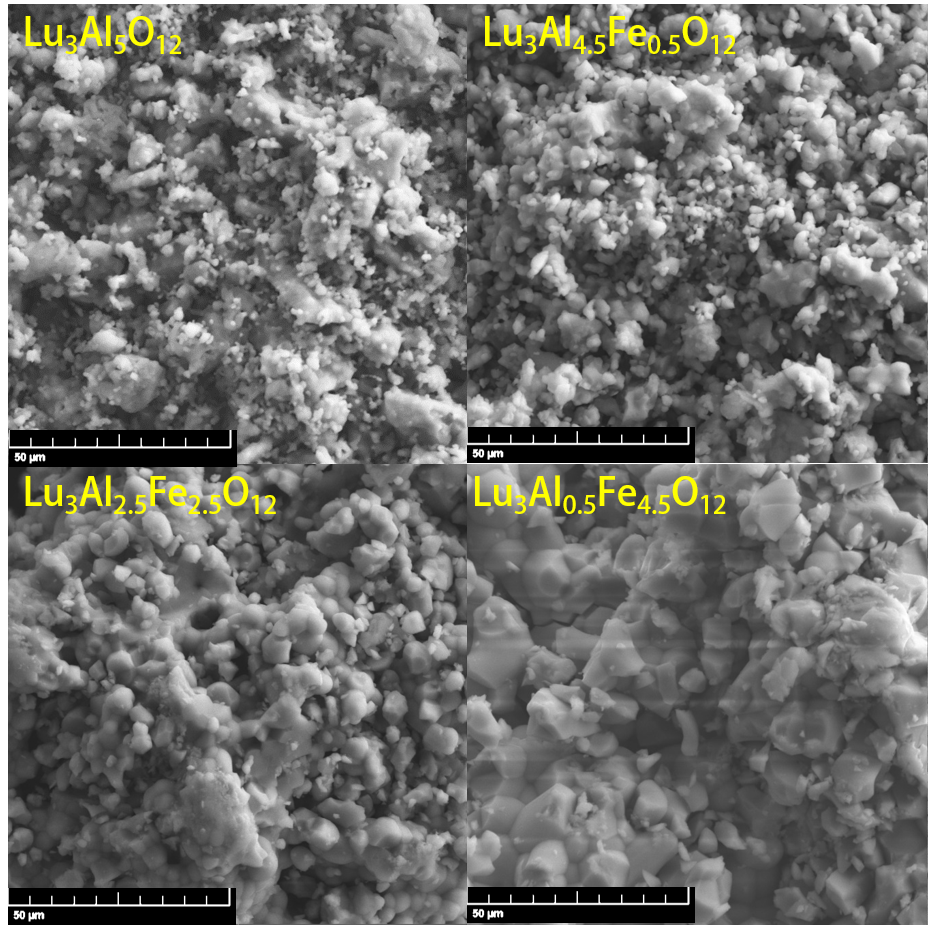
\includegraphics[width=12cm]{Kap5/sec20k.png}%
    \caption{Micrografías con electrones secundarios a 90.000 aumentos para los
    materiales \ce{Lu3Al_{5-X}Fe_{x}O12}:\ce{Ce^{3+}} con x=0.0, 0.5, 2.5
    }\label{fig:sec90}
\end{figure}

En la Figura \ref{fig:sec90} se muestran las micrografías a 90.000 aumentos, en donde, se
observa poco espacio entre partículas, lo que permite confirmar que el proceso
de prensado para obtener las pastillas de cada muestra favoreció la cinética de
densificación. Sin embargo, no se obtuvo la misma densificación para todas las
muestras debido a variación en la composición química y el tamaño de partícula
de los precursores \cite{MoralesRivera2019}. El proceso de prensado ayudó en la difusión y reacción
entre los precursores permitiendo la formación de la fase cristalina deseada y
llevo a una reducción en la temperatura y tiempo de sinterización \cite{Kang2005}.\\

Por medio del software ImageJ se determinó el tamaño promedio aproximado de
partícula de las muestras del sistema \ce{Lu3Al_{5-X}Fe_{x}O12}:\ce{Ce^{3+}} con x = 0.0, 0.5, 2.5 y
4.5 obtenidos por el método cerámico utilizando las imágenes tomadas a 20.000
aumentos. En el Anexo \ref{AnexoD} se muestran las distribuciones aproximadas de tamaño de
partícula obtenidos para cada uno de los materiales del sistema. En donde, se
observó un aumento del tamaño de las partículas a medida que se aumentó el
dopaje con \ce{Fe^{3+}} (ver Figura \ref{fig:sec90}). Por lo tanto se puedo determinar que el tamaño de partícula
aumentó cuando el \ce{Fe^{3+}} se incorporo dentro de la estructura cristalina del 
granate LUAG, por lo tanto, se evidencia una relación entre el tamaño de grano con los radios iónicos. 
Se sabe que el radio iónico del \ce{Fe^{3+}} es mayor que el del \ce{Al^{3+}}. También se identifica que el
tamaño de partícula presenta un comportamiento similar al tamaño de cristalito
calculado mediante el refinamiento Rietveld de los patrones obtenidos por DRX \cite{Akhtar2017a}.
\\

\begin{figure}[h]
    \centering%

    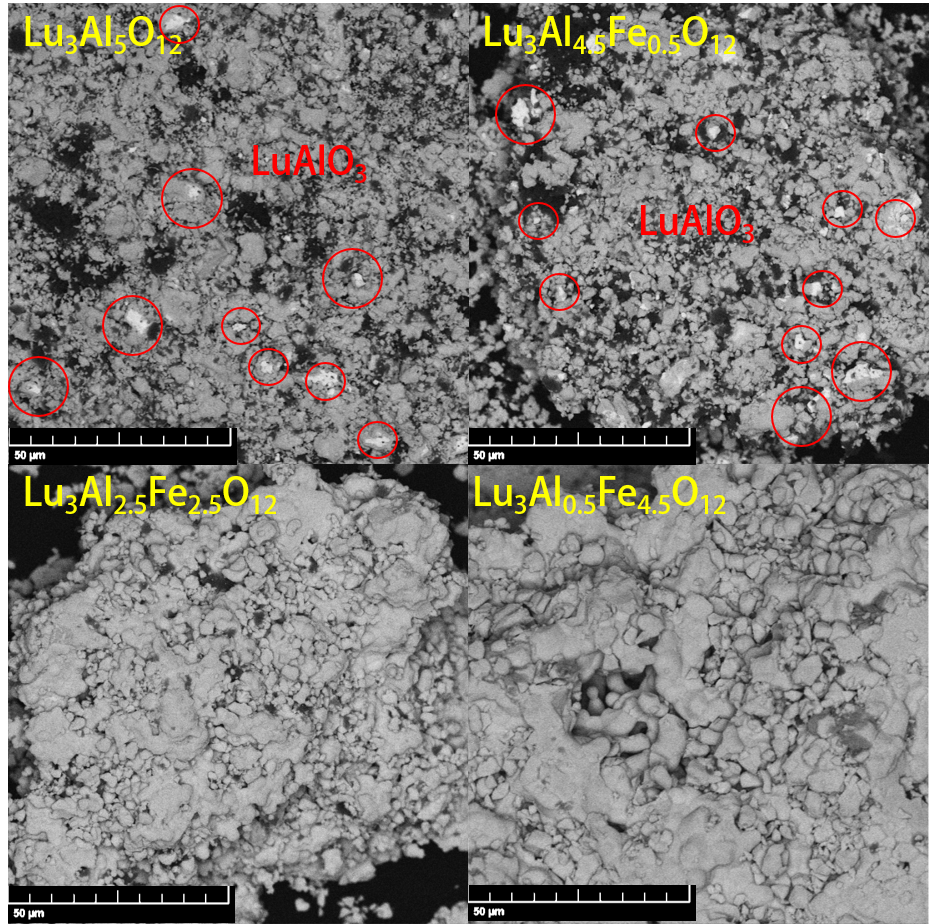
\includegraphics[width=12cm]{Kap5/ret10k.png}%
    \caption{Micrografías con electrones retrodispersados a 10k aumentos. 
    En círculos rojos se señala la presencia de la fase secundaria (\ce{LuAlO2}) }
    \label{fig:ret10}
\end{figure}

En la Figura \ref{fig:ret10} se presentan las micrografías con electrones retro dispersados,
en donde, se puede apreciar que para los materiales \ce{Lu3Al5O12} y
\ce{Lu3Al_{4.5}Fe_{0.5}O12} se observan partículas con una tonalidad más clara que se
asocia con la presencia de la fase secundaria \ce{LuAlO3} que se identificó mediante
la difracción de rayos X y el refinamiento Rietveld, igualmente se confirma la
pureza para $x\leq 2.5$, mediante las micrografías de los materiales
\ce{Lu3Al_{2.5}Fe_{2.5}O12} y \ce{Lu3Al_{0.5}Fe_{4.5}O12}, donde, se tiene uniformidad en la
composición de todas las partículas.\\


\begin{figure}[t]
    \centering%

    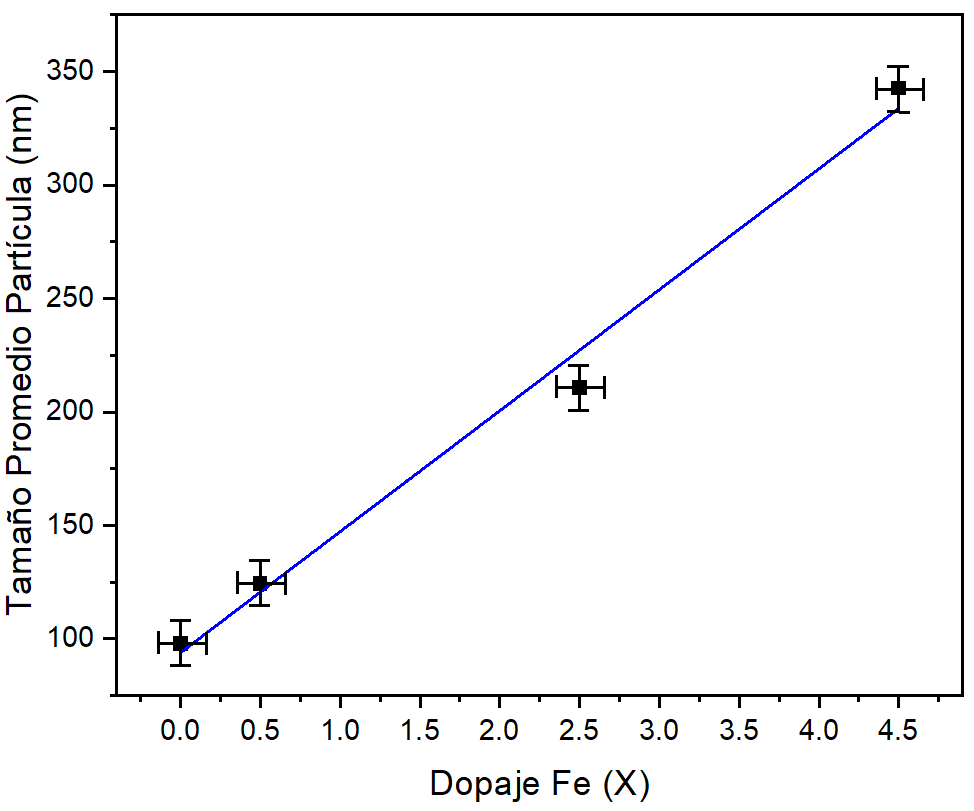
\includegraphics[width=12cm]{Kap5/TamPar.png}%
    \caption{Tamaño de partícula en función del dopaje con \ce{Fe^{3+}}
    }\label{fig:tamfe}
\end{figure}

\begin{table}[h]
    \caption{Porcentaje atómico teórico y experimental obtenido de los resultados de EDX}
    \label{tab:porce}
    %\resizebox{\textwidth}{!}{%
    \begin{tabular}{cccccc}
    \hline
    \multirow{2}{*}{Valor   de x} & \multirow{2}{*}{Formula} & \multicolumn{4}{c}{\% Atomico Teorico   (Experimental)} \\ \cline{3-6} 
        &                             & Lu        & Al          & Fe         & O         \\ \hline
    0.0 & \ce{Lu3Al5O12}              & 15(23.63) & 25.0(26.79) & -          & 60(49.58) \\
    0.5 & \ce{Lu3Al_{4.5}Fe_{0.5}O12}  & 15(16.47) & 22.5(20.16) & 2.5(2.4)   & 60(60.97) \\
    2.5 & \ce{Lu3Al_{2.5}Fe_{2.5}O12} & 15(22.40) & 12.5(10.43) & 12.5(13.2) & 60(53.96) \\
    4.5 & \ce{Lu3Al_{4.5}Fe_{0.5}O12} & 15(20.81) & 2.5(2.63)   & 22.5(27.1) & 60(49.44) \\ \hline
    \end{tabular}%
    %}
\end{table}

Mediante los resultados del análisis semicuantitativo de EDX (ver Anexo \ref{edx}) para las muestras con x=0.0, 0.5, 2.5 y 4.5
se construyó la Tabla \ref{tab:porce} donde se presentan los porcentajes atómicos comparados
con los porcentajes teóricos según la fórmula química. En la Tabla \ref{tab:proporcion} se lista 
la relación lutecio-hierro con el fin de observar mejor la diferencia, de ahí
se puede inferir que el proceso de sinterización fue adecuado, ya que permitió
obtener materiales con una relación aproximada a lo esperado.\\

\begin{table}[h]
    \caption{Proporción Fe/Lu teórica y experimental mediante los resultados de EDX}
    \label{tab:proporcion}
    %\resizebox{\textwidth}{!}{%
    \begin{tabular}{ccccc}
    \hline
    \multirow{2}{*}{Valor de x} & \multirow{2}{*}{Formula} & \multicolumn{2}{c}{Proporción Fe/Al} & \multirow{2}{*}{Diferencia} \\ \cline{3-4}
        &                             & Teórica & Experimental &      \\ \hline
    0.0 & \ce{Lu3Al5O12}              & 0.00    & 0.00         & 0.00 \\
    0.5 & \ce{Lu3Al_{4.5}Fe_{0.5}O12}  & 0.11    & 0.12         & 0.01 \\
    2.5 & \ce{Lu3Al_{2.5}Fe_{2.5}O12} & 1.00    & 1.27         & 0.27 \\
    4.5 & \ce{Lu3Al_{4.5}Fe_{0.5}O12} & 9.00    & 10.31        & 1.31 \\ \hline
    \end{tabular}%
    %}
\end{table}


